% Soubory musí být v kódování, které je nastaveno v příkazu \usepackage[...]{inputenc}

\documentclass[%        Základní nastavení
%  draft,    				  % Testovací překlad
  12pt,       				% Velikost základního písma je 12 bodů
  a4paper,    				% Formát papíru je A4
  oneside,      			% Jednostranný tisk
	%twoside,      			% Dvoustranný tisk (kapitoly a další důležité části tedy začínají na lichých stranách)
	unicode						% Záložky a metainformace ve výsledném  PDF budou v kódování unicode
]{report}				    	% Dokument třídy 'zpráva', vhodná pro sazbu závěrečných prací s kapitolami

\usepackage[				% Nastavení geometrie stránky
	bindingoffset=10mm,		% Hřbet pro vazbu
	hmargin={25mm,25mm},	% Vnitřní a vnější okraj
	vmargin={25mm,34mm},	% Horní a dolní okraj
	footskip=17mm,			  % Velikost zápatí
	nohead,					      % Bez záhlaví
	marginparsep=2mm,		  % Vzdálenost marginálií
	marginparwidth=18mm,	% Šířka marginálií
]{geometry}

\usepackage{sectsty}
	%přetypuje nadpisy všech úrovní na bezpatkové, kromě \chapter, která je přenastavena zvlášť v thesis.sty
	\allsectionsfont{\sffamily}

\usepackage{graphicx} % Balíček 'graphicx' pro vkládání obrázků
											% Nutné pro vložení logotypů školy a fakulty

\usepackage[          % Balíček 'acronym' pro sazby zkratek a symbolů
	nohyperlinks				% Nebudou tvořeny hypertextové odkazy do seznamu zkratek
]{acronym}						
											% Nutné pro použití prostředí 'acronym' balíčku 'thesis'

\usepackage[
	breaklinks=true,		% Hypertextové odkazy mohou obsahovat zalomení řádku
	hypertexnames=false % Názvy hypertext. odkazů budou tvořeny nezávisle na názvech TeXu
]{hyperref}						% Balíček 'hyperref' pro sazbu hypertextových odkazů
											% Nutné pro použití příkazu 'pdfsettings' balíčku 'thesis'

\usepackage{pdfpages} % Balíček umožňující vkládat stránky z PDF souborů
                      % Nutné při vkládání titulních listů a zadání přímo
                      % ve formátu PDF z informačního systému

\usepackage{enumitem} % Balíček pro nastavení mezerování v odrážkách
  \setlist{topsep=0pt,partopsep=0pt,noitemsep} % konkrétní nastavení

\usepackage{cmap} 		% Balíček cmap zajišťuje, že PDF vytvořené `pdflatexem' je
											% plně "prohledávatelné" a "kopírovatelné"

%\usepackage{upgreek}	% Balíček pro sazbu stojatých řeckých písmem
											%% např. stojaté pí: \uppi
											%% např. stojaté mí: \upmu (použitelné třeba v mikrometrech)
											%% pozor, grafická nekompatibilita s fonty typu Computer Modern!
                      
\usepackage{amsmath} %balíček pro sabu náročnější matematiky                 

\usepackage{dirtree}	% sazba adresářové struktury
                      % vhodné pro prezentaci obsahu elektronické přílohy (např. CD)

\usepackage{subcaption}
\usepackage{float}
\usepackage{amsfonts}

\usepackage[formats]{listings}	% Balíček pro sazbu zdrojových textů
\lstset{              % nastavení
%	Definice jazyka použitého ve výpisech
%    language=[LaTeX]{TeX},	% LaTeX
%	language={Matlab},		% Matlab
	language={Python},           % jazyk Python
    basicstyle=\ttfamily,	% definice základního stylu písma
    tabsize=2,			% definice velikosti tabulátoru
    inputencoding=utf8,         % pro soubory uložené v kódování UTF-8
		columns=fixed,  %fixed nebo flexible,
		fontadjust=true %licovani sloupcu
    extendedchars=true,
    literate=%  definice symbolů s diakritikou
    {á}{{\'a}}1
    {č}{{\v{c}}}1
    {ď}{{\v{d}}}1
    {é}{{\'e}}1
    {ě}{{\v{e}}}1
    {í}{{\'i}}1
    {ň}{{\v{n}}}1
    {ó}{{\'o}}1
    {ř}{{\v{r}}}1
    {š}{{\v{s}}}1
    {ť}{{\v{t}}}1
    {ú}{{\'u}}1
    {ů}{{\r{u}}}1
    {ý}{{\'y}}1
    {ž}{{\v{z}}}1
    {Á}{{\'A}}1
    {Č}{{\v{C}}}1
    {Ď}{{\v{D}}}1
    {É}{{\'E}}1
    {Ě}{{\v{E}}}1
    {Í}{{\'I}}1
    {Ň}{{\v{N}}}1
    {Ó}{{\'O}}1
    {Ř}{{\v{R}}}1
    {Š}{{\v{S}}}1
    {Ť}{{\v{T}}}1
    {Ú}{{\'U}}1
    {Ů}{{\r{U}}}1
    {Ý}{{\'Y}}1
    {Ž}{{\v{Z}}}1
}

%%%%%%%%%%%%%%%%%%%%%%%%%%%%%%%%%%%%%%%%%%%%%%%%%%%%%%%%%%%%%%%%%
%%%%%%      Definice informací o dokumentu             %%%%%%%%%%
%%%%%%%%%%%%%%%%%%%%%%%%%%%%%%%%%%%%%%%%%%%%%%%%%%%%%%%%%%%%%%%%%

% V tomto souboru se nastavují téměř veškeré informace, proměnné mezi studenty:
% jméno, název práce, pohlaví atd.
% Tento soubor je SDÍLENÝ mezi textem práce a prezentací k obhajobě -- netřeba něco nastavovat na dvou místech.

\usepackage[
%%% Z následujících voleb jazyka lze použít pouze jednu
  czech-english,		% originální jazyk je čeština, překlad je anglicky (výchozí)
  %english-czech,	% originální jazyk je angličtina, překlad je česky
  %slovak-english,	% originální jazyk je slovenština, překlad je anglicky
  %english-slovak,	% originální jazyk je angličtina, překlad je slovensky
%
%%% Z následujících voleb typu práce lze použít pouze jednu
  semestral,		  % semestrální práce (nesází se abstrakty, prohlášení, poděkování) (výchozí)
  %bachelor,			%	bakalářská práce
  %master,			  % diplomová práce
  %treatise,			% pojednání o disertační práci
  %doctoral,			% disertační práce
%
%%% Z následujících voleb zarovnání objektů lze použít pouze jednu
%  left,				  % rovnice a popisky plovoucích objektů budou zarovnány vlevo
	center,			    % rovnice a popisky plovoucích objektů budou zarovnány na střed (vychozi)
%
]{thesis}   % Balíček pro sazbu studentských prací


%%% Jméno a příjmení autora ve tvaru
%  [tituly před jménem]{Křestní}{Příjmení}[tituly za jménem]
% Pokud osoba nemá titul před/za jménem, smažte celý řetězec '[...]'
\author[Bc.]{Viktor}{Slezák}

%%% Identifikační číslo autora (VUT ID)
\butid{203745}

%%% Pohlaví autora/autorky
% (nepoužije se ve variantě english-czech ani english-slovak)
% Číselná hodnota: 1...žena, 0...muž
\gender{0}

%%% Jméno a příjmení vedoucího/školitele včetně titulů
%  [tituly před jménem]{Křestní}{Příjmení}[tituly za jménem]
% Pokud osoba nemá titul před/za jménem, smažte celý řetězec '[...]'
\advisor[Ing.]{Matěj}{Ištvánek}

%%% Jméno a příjmení oponenta včetně titulů
%  [tituly před jménem]{Křestní}{Příjmení}[tituly za jménem]
% Pokud osoba nemá titul před/za jménem, smažte celý řetězec '[...]'
% Nastavení oponenta se uplatní pouze v prezentaci k obhajobě;
% v případě, že nechcete, aby se na titulním snímku prezentace zobrazoval oponent, pouze příkaz zakomentujte;
% u obhajoby semestrální práce se oponent nezobrazuje (jelikož neexistuje)
% U dizertační práce jsou typicky dva až tři oponenti. Pokud je chcete mít na titulním slajdu, prosím ručně odkomentujte a upravte jejich jména v definici "VUT title page" v souboru thesis.sty.
\opponent[doc.\ Mgr.]{Křestní}{Příjmení}[Ph.D.]

%%% Název práce
%  Parametr ve složených závorkách {} je název v originálním jazyce,
%  parametr v hranatých závorkách [] je překlad (podle toho jaký je originální jazyk).
%  V případě, že název Vaší práce je dlouhý a nevleze se celý do zápatí prezentace, použijte příkaz
%  \def\insertshorttitle{Zkác.\ náz.\ práce}
%  kde jako parametr vyplníte zkrácený název. Pokud nechcete zkracovat název, budete muset předefinovat,
%  jak se vytváří patička slidu. Viz odkaz: https://bit.ly/3EJTp5A
\title[Light animations for the Spectoda system based on the analysis of parameters from music recordings]{Světelné animace pro systém Spectoda na základě analýzy parametrů z hudebních nahrávek}

%%% Označení oboru studia
%  Parametr ve složených závorkách {} je název oboru v originálním jazyce,
%  parametr v hranatých závorkách [] je překlad
\specialization[Audio engineering]{Audio inženýrství}

%%% Označení ústavu
%  Parametr ve složených závorkách {} je název ústavu v originálním jazyce,
%  parametr v hranatých závorkách [] je překlad
%\department[Department of Control and Instrumentation]{Ústav automatizace a měřicí techniky}
%\department[Department of Biomedical Engineering]{Ústav biomedicínského inženýrství}
%\department[Department of Electrical Power Engineering]{Ústav elektroenergetiky}
%\department[Department of Electrical and Electronic Technology]{Ústav elektrotechnologie}
%\department[Department of Physics]{Ústav fyziky}
%\department[Department of Foreign Languages]{Ústav jazyků}
%\department[Department of Mathematics]{Ústav matematiky}
%\department[Department of Microelectronics]{Ústav mikroelektroniky}
%\department[Department of Radio Electronics]{Ústav radioelektroniky}
%\department[Department of Theoretical and Experimental Electrical Engineering]{Ústav teoretické a experimentální elektrotechniky}
\department[Department of Telecommunications]{Ústav telekomunikací}
%\department[Department of Power Electrical and Electronic Engineering]{Ústav výkonové elektrotechniky a elektroniky}

%%% Označení fakulty
%  Parametr ve složených závorkách {} je název fakulty v originálním jazyce,
%  parametr v hranatých závorkách [] je překlad
%\faculty[Faculty of Architecture]{Fakulta architektury}
\faculty[Faculty of Electrical Engineering and~Communication]{Fakulta elektrotechniky a~komunikačních technologií}
%\faculty[Faculty of Chemistry]{Fakulta chemická}
%\faculty[Faculty of Information Technology]{Fakulta informačních technologií}
%\faculty[Faculty of Business and Management]{Fakulta podnikatelská}
%\faculty[Faculty of Civil Engineering]{Fakulta stavební}
%\faculty[Faculty of Mechanical Engineering]{Fakulta strojního inženýrství}
%\faculty[Faculty of Fine Arts]{Fakulta výtvarných umění}
%
%Nastavení logotypu (v hranatych zavorkach zkracene logo, ve slozenych plne):
\facultylogo[logo/FEKT_zkratka_barevne_PANTONE_CZ]{logo/UTKO_color_PANTONE_CZ}

%%% Rok odevzdání práce
\graduateyear{2023}
%%% Akademický rok odevzdání práce
\academicyear{2023/24}

%%% Datum obhajoby (uplatní se pouze v prezentaci k obhajobě)
\date{11.\,11.\,1980} 

%%% Místo obhajoby
% Na titulních stránkách bude automaticky vysázeno VELKÝMI písmeny (pokud tyto stránky sází šablona)
\city{Brno}

%%% Abstrakt
\abstract[%
In this paper, is explored the field of Music Information Retrieval. Based on the knowledge acquired, a system structure for generating animations from parameters of a music recording is proposed. Furthermore, the possibilities for extracting these parameters are described and compared.
]{%
V práci je prozkoumána problematika oboru Music information retrieval. Na základě získaných znalostí je navržena struktura systému pro generování animací z parametrů hudební nahrávky. Dále jsou popsány a porovnány možnosti jak tyto parametry extrahovat.
}

%%% Klíčová slova
\keywrds[%
MIR, feature extraction, audio analysis, animation generator
]{%
MIR, extrakce parametrů, audio analýza, generátor animací
}

%%% Poděkování
\acknowledgement{%
Rád bych poděkoval vedoucímu diplomové práce
panu Ing. Matěj Ištvánek\ za odborné vedení,
konzultace, trpělivost a~podnětné návrhy k~práci.
}%  % do tohoto souboru doplňte údaje o sobě, druhu práce, názvu...

\usepackage[utf8]		  %	Kódování zdrojových souborů je UTF-8
	{inputenc}					% Balíček pro nastavení kódování zdrojových souborů
\usepackage{fontspec}
%%%%%%%%%%%%%%%%%%%%%%%%%%%%%%%%%%%%%%%%%%%%%%%%%%%%%%%%%%%%%%%%%%%%%%%%

%%%%%%%%%%%%%%%%%%%%%%%%%%%%%%%%%%%%%%%%%%%%%%%%%%%%%%%%%%%%%%%%%%%%%%%%
%%%%%%     Nastavení polí ve Vlastnostech dokumentu PDF      %%%%%%%%%%%
%%%%%%%%%%%%%%%%%%%%%%%%%%%%%%%%%%%%%%%%%%%%%%%%%%%%%%%%%%%%%%%%%%%%%%%%
%% Při načteném balíčku 'hyperref' lze použít příkaz '\pdfsettings':
\pdfsettings
%  Nastavení polí je možné provést také ručně příkazem:
%\hypersetup{
%  pdftitle={Název studentské práce},    	% Pole 'Document Title'
%  pdfauthor={Autor studenstké práce},   	% Pole 'Author'
%  pdfsubject={Typ práce}, 						  	% Pole 'Subject'
%  pdfkeywords={Klíčová slova}           	% Pole 'Keywords'
%}
%%%%%%%%%%%%%%%%%%%%%%%%%%%%%%%%%%%%%%%%%%%%%%%%%%%%%%%%%%%%%%%%%%%%%%%

\pdfmapfile{=vafle.map}

%%%%%%%%%%%%%%%%%%%%%%%%%%%%%%%%%%%%%%%%%%%%%%%%%%%%%%%%%%%%%%%%%%%%%%%
%%%%%%%%%%%       Začátek dokumentu               %%%%%%%%%%%%%%%%%%%%%
%%%%%%%%%%%%%%%%%%%%%%%%%%%%%%%%%%%%%%%%%%%%%%%%%%%%%%%%%%%%%%%%%%%%%%%
\begin{document}
\pagestyle{empty} %vypnutí číslování stránek

%%% Vložení desek -- od září 2021 na žádost fakulty nepoužíváno
\includepdf[pages=1]%  buďto generovaných informačním systémem
  {pdf/semestral-desky}% název souboru nesmí obsahovat mezery!
%%% NEBO vytvoření desek z balíčku
%%\makecover
%%%
%\oddpage % při dvojstranném tisku přidá prázdnou stránku
%% kazdopádně ale:
%\setcounter{page}{1} %resetovaní čítače stránek -- desky do číslování nezahrnujeme

%% Vložení titulního listu
\includepdf[pages=1]%    buďto generovaného informačním systémem
  {pdf/semestral-titulka}% název souboru nesmí obsahovat mezery!
%% NEBO vytvoření titulní stránky z balíčku
%\maketitle
%%
\oddpage  % při dvojstranném tisku se přidá prázdná stránka
   
%% Vložení zadání
\includepdf[pages=1]%   buďto generovaného informačním systémem
  {pdf/semestral-zadani}% název souboru nesmí obsahovat mezery!
%% NEBO lze vytvořit prázdný list příkazem ze šablony
%\patternpage{}%
%	{\sffamily\Huge\centering ZDE VLOŽIT LIST ZADÁNÍ}%
%	{\sffamily\centering Z~důvodu správného číslování stránek}
%%
\oddpage% při dvojstranném tisku se přidá prázdná stránka

%% Vysázení stránky s abstraktem
%\makeabstract

% Vysázení stránky s rozšířeným abstraktem
% (pokud píšete práci v češtině či slovenštině, vložení rozšířeného abstraktu zrušte;
%  pro semestrální projekt také není potřeba rozšířený abstrakt uvádět)
%% Vysázení stránky s rozšířeným abstraktem
% (týká se pouze bc. a dp. prací psaných v angličtině, viz Směrnice rektora 72/2017)
\cleardoublepage
\noindent
{\large\sffamily\bfseries\MakeUppercase{Rozšířený abstrakt}}
\\
Výtah ze směrnice rektora 72/2017:\\
\emph{Bakalářská a diplomová práce předložená v angličtině musí obsahovat rozšířený abstrakt v češtině
nebo slovenštině (čl. 15). To se netýká studentů, kteří studují studijní program akreditovaný v
angličtině.}
(čl. 3, par. 7)\\
\emph{Nebude-li vnitřní normou stanoveno jinak, doporučuje se rozšířený abstrakt o rozsahu přibližně 3
normostrany, který bude obsahovat úvod, popis řešení a shrnutí a zhodnocení výsledků.}
(čl. 15, par. 5) 

%%% Vysázení citace práce
\makecitation

%%% Vysázení prohlášení o samostatnosti
% \makedeclaration

%%% Vysázení poděkování
% \makeacknowledgement

%%% Vysázení obsahu
\tableofcontents

%%% Vysázení seznamu obrázků
% (vynechejte, pokud máte dva nebo méně obrázků)
\listoffigures

%%% Vysázení seznamu tabulek
% (vynechejte, pokud máte dvě nebo méně tabulek)
\listoftables

%%% Vysázení seznamu výpisů kódu
% (vynechejte, pokud máte dva nebo méně výpisů)
%\lstlistoflistings

\cleardoublepage\pagestyle{plain}   % zapnutí číslování stránek

%Pro vkládání kapitol i příloh používejte raději \include než \input
%%% Vložení souboru 'text/uvod.tex' s úvodem
\chapter*{Úvod}
\phantomsection
\addcontentsline{toc}{chapter}{Úvod}


Úvod studentské práce, např\,\dots

Nečíslovaná kapitola Úvod obsahuje \uv{seznámení} čtenáře s~problematikou práce.
Typicky se zde uvádí:
(a) do jaké tematické oblasti práce spadá, (b) co jsou hlavní cíle celé práce a (c) jakým způsobem jich bylo dosaženo.
Úvod zpravidla nepřesahuje jednu stranu.
Poslední odstavec Úvodu standardně představuje základní strukturu celého dokumentu.

Tato práce se věnuje oblasti \acs{DSP} (\acl{DSP}), zejména jevům, které nastanou při nedodržení Nyquistovy podmínky pro \ac{symfvz}.%
\footnote{Tato věta je pouze ukázkou použití příkazů pro sazbu zkratek.}

Šablona je nastavena na \emph{dvoustranný tisk}.
Nebuďte překvapeni, že ve vzniklém PDF jsou volné stránky.
Je to proto, aby důležité stránky jako např.\ začátky kapitol začínaly po vytisknutí a svázání vždy na pravé straně.
%
Pokud máte nějaký závažný důvod sázet (a~zejména tisknout) jednostranně, nezapomeňte si přepnout volbu \texttt{twoside} na \texttt{oneside}!

%%% Vložení souboru 'text/reseni' s popisem řešení práce
% (rozdělte na více souborů či kapitol, pokud je vhodné)
\chapter{Teorie}

Semestrální práce se zejména zabývá problematikou \acs{MIR}. Popsánou v kapitole (!doplnit kapitolu!).
Důležitou roli zde hraje i úvaha nad realizací světelných animací.
Je důležité aby bylo přemýšleno nad principem reakce světelných animací na hudbu.
Nabízejí se otázky jak by měla daná animace reagovat na konkrétní děj skladby.
Jakým způsobem navrhnout strukturu \dots

V táto části je popsána teorie zpracování hudební nahrávky pomocí známých algoritmů jako je například \acs{FFT} (\acl{FFT}) 
či nabízené možnosti strojového učení. Struktura a možnosti systému Spectoda pro generování interaktivních světelných animací.
Uměleckou částí, jak by měla animace prezentovat hudbu.

\section{MIR - Music information retrieval}
    Music information retrieval je interdisciplinární vědní obor sostředící se na získávání infromací z hudebních nahrávek.
    Jsou zde kombinovány znalosti mnoha oborů jako jsou muzikologie, psychoakustika, strojové učení, zpracování signálů a další. 
    

    Výstup jeho výzkumu je využíván populárními technologiemi. 
    Jednou z aplikací je personalizované doporučování hudebních skladeb, která se nachází v moderních streamovacích platformách.
    Další využítí je v programech pro mixování hudby používaných diskžokeji k plynulejší práci díky alanýze tempe a klíčových částí skladby.
    Tyto technologie se nachází v mnoha dalších aplikacích a s šířením se digitálního audia jejich důležitost stále poroste.
    \cite{lidy09:448[TUW-181186]}\cite{a_new_companion_to_digital_humanities}
    
    \subsection{Historie}
    \acs*{MIR} se začíná objevovat koncem devatenáctého a začátkme dvacátého století s příchodem moderních statistických metod.
    V některých univerzitách tyto statistické metody začínají aplikovat na hudebu.
    Ze začátku díky špatné dostupnosti počítačů se jedná spíše o ruční přepisování tabulatur přímo z hudebních partitur.
    Následně se ze zjištěných rysů snažili specifikovat stylové chrakteristiky.  
    S příchodem počítačů do výzkumných laboratoří v letech 1960 až 1970 se začalo více soutředit na počítačovou analýzu hudeby.
    V těchto letech se poprvé začaly objevoat nyní známé termíny jako \uv{\it computational musicology} a \uv{\it music information retrieval}
    První oblastí výzkumu bylo získávání rytmu hudbení nahrávky a z důvodu nízké popularity se výzkum zpomalil.
    Tento trend následoval až do roku 1990 kdy vázkumu \acs*{MIR} pomohly dvě věci.
    První z nich bylo velké zvětšování lehce dostupné hudby a druhým z důležitých bodů byl nárůst výpočetního výkonu počítačů.
    Díky těmto bodům se stal výzkum dostupnější a jednodužší na realizaci.

    Poté v říjnu roku 2000 bylo uspořádáno první mezinárodní symposium soustředící se na \acs*{MIR}.
    Následně díky těmto pokrokům vznika celosvětová skupina \acs{ISMIR} (\acl{ISMIR}).
    Zanedlouho naté vznikla další skupina \acs{MIREX} (\acl{MIREX}). Jedná se o skupinu vědců která se schází pravidelně každý rok a řeší problematiku \acs{MIR}.
    
   \subsection{Řetězec zpracování - pipeline}

    Téměř standardně využívaný řetězec procesů v aplikacíc \acs{MIR} je popsána níže. 

    Jako vstupní data se využívají zejména hudební informace v digitální potobě.
    Tyto data se rozlišují do více typů. Mohou to být obrázky představující digitální formu zápisu hudby pomocí symbolů (not).
    Dalším možným typem je "digitální hudba", představovaná zápisem v \acs{MIDI} notách.
    V této práci budou jako vstupní data yvužívány digitální hudební nahrávky ("digitální audio"). 

    Pokud jsou vstupní data komplexní na začátku je v řetězci zařezen blok předzpracování, která se stará o komprimaci vstupních singálů.
    U hudebních signálů se jedná například o konverzi stereo signálů na mono signál
    a jeho následnou komprimaci popsanou více v bodě 
    %TODO: odkaz na bod audio

    Dalším bodem v řetězci je extrakce vlastností signálu. 
    Zde je je nastaven poměr mezi vlastnostmi důležitými pro strojové učení lidskou expertní znalost.
    Poměr mezi těmito vlastnostmi závisí na aplikaci pro kterou je algoritmus určen.
    Ná základě získaných vlastností je nastavena struktura algoritmu pro odvození výsldných parametrů.

\begin{figure}[H]
    \centering
    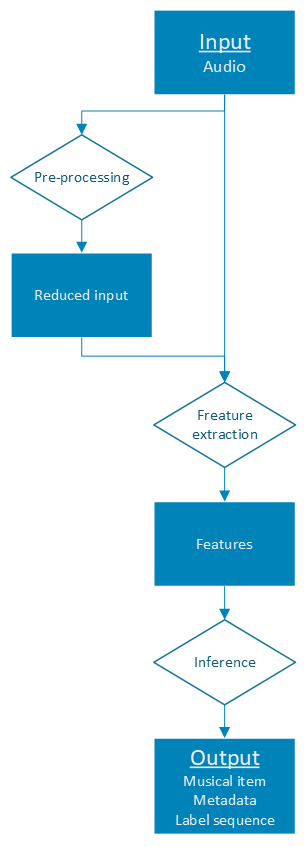
\includegraphics[width = 0.4\linewidth]{obrazky/MIR-diagram.png}
    \caption{Řetězec procesů MIR \cite{a_new_companion_to_digital_humanities}}
    \label{fig:MIR_diagram}
\end{figure}

    Zpracování audio signálů je již dvě desetilétí hlavním trendem výzkumu \acs*{MIR}.
    Je to přirození tím, že zde není téměř žádná přirozená hranice a je možné téměř vše.
    Právní podmínky jsou zde příznivé a vědecké instituce nemají problém pro svou práci získat velké množství materiálu chráněného autorským právem.
    Z důvodu velké komplexsnosti vstupních signálů se využívá několik technik komprimaca signálů kterými jsou. 
    Slučování vícekanálových nahrávek do mono sginálu. Převzorkování signálu na nižší vzorkovací kmitočty,
    a rozložení signálu na krátké překrývající se úseky ze kterých mohou být nezávisle extrahovány jejich vlastnosti. 
    Výsledkem je kolekce paralelně složených sekvencí hodnot vlastností, které se následně použijí pro odvozování (inference).

  \begin{table}[H]
    \centering
    \begin{tabular}{|p{0.07\linewidth} | p{0.31\linewidth} | p{0.27\linewidth} | p{0.25\linewidth}|}
        \hline
        {\bf Data}                 & {\bf Vyhledávání informací} & {\bf Klasifikace a odhad} & {\bf Sekvenční značení}\\
        \hline
        Audio                      & Identifikace skladby,
                                     Řazení,
                                     Měření podobnosti,
                                     Získání otisku,
                                     Generování seznamu skladeb
                                   & Identifikace umělce a skladatele,
                                     Žánr a nálada,
                                     Určení tempa
                                   & Extrakce melodie,
                                     Odhad akordů,
                                     Detekce nástupů,
                                     Segmentace                   \\
        \hline
    \end{tabular}
    \caption{Typické procesy na základně vstupních a výstupních dat.}
    \label{tab:MIR_typicke_procesy}
  \end{table}

  %TODO: současné problémy


  \section{Parametrizace hudebních nahrávek}
  V této kapitole je popsán audio signál. Jak vzniká, jeho reprezentace v číslicovám zpracování a základní principy práce s audiosignálem.
  V bodech \ref{sec:Frekvence} až \ref{sec:Barva} jsou popsány parametry získávané z audio signálu. %TODO: doplnit správné reference
  Získané parametry slouží pro přesnější popis skladby. \cite{fundamental_of_music_processing}

  \subsection{Reprezentace audio signálů}
  Hudba může být reprezentována spoustou forem. 
  Jako tradiční médium pro její ukládání ještě před vznikem záznamu sloužily vždy noty a další typy zápisů pomocí symbolů.
  Výsledné hudební dílo ale představuje mnohem více než počáteční notový zápis.
  Každý hudebník a hudební nástroj do skladby dodává svou unikátnost.
  Při hře se noty začnou proměňovat v harmonické zvuky, hladké melodie a nástroje vzájemně rezonují. 
  Každý z hudebníků do skladby přináší svou interptretaci. Jinak reagují na tempo zvýrazňují odlišné noty a liší se jejich artikulace.
  Všechny tyto proměnné ve výsledku způsobují, že dílo není jen mechanické přehrání napsané partitury.
  Jeho součástí se stává unikátní přednes.

  Při pohledu z fyzikálního hlediska důsledkem interpretace díla vznikají zvukové vlny šířící se vzduchem.
  Tyto vlny jsou reprezentovány kmítáním atomů plynu způsobující změny tlaku svým zhušťováním a zřěďováním. Při vlnění nedochází k přenosu hmotných částit.
  Záznamem šířících se zvukových vln získáváme audio signál.
  Pojmem audio je označován řetězec sloužící k záznamu, přenosu a reprodukci zvuků v mezích lidského slyšení. 
  Avšak v audio signálu se už nenachází přesná reprezentace not a jejich paramterů jako jsou čas nástupu, tón, délka trvání, dynamika.
  Díky tomu je analýza hudebních signálů obtížným úkolem a je ovlivněna reprezentací interpreta akustikou prostoru a vnímáním posluchače.
  Popsanými problémy se zabývá samostatný vědní obor s názvem psychoakustika.
  Nejdůležitějšími parametry audio signálu které jsou podrobně popsány níže definujeme: frekvence, výška tónu, dynamika, intenzita, hlasitost a také barva.


  \subsection{Časová oblast}
  Základní reprezentací audio signálu je tzv. zobrazení v \textbf{časové oblasti}.
  V časové oblasti číslicový signál představují vzorky. Jednotlivé vzorky udávají hodnotu signálu v daném čase.
  Počet vzorků nám určuje vzorkovací frekvence signálu. Důležé pravidlo pro vzorkování signálu je popsáno rovnicí č. \ref*{rov:vzorkovaci_teorem}
  
  \begin{equation}
    f_{vz} > 2 * f_{max}
    \label{rov:vzorkovaci_teorem}
  \end{equation}

  kde $f_{vz}$ je vzorkovací frekvence a $f_{max}$ je maximální frekvence v audio signálu.  
  Pokud jednotlivé vzorky zobrazíme graficky získáme průběh amplitudy signálu viz obrázek č.\ref*{fig:Waveform}

  \begin{figure}[H]
    \centering
    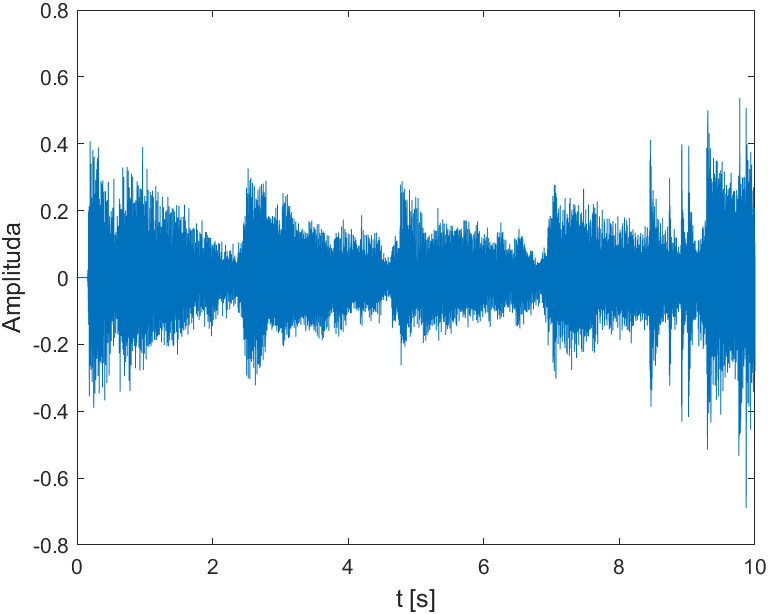
\includegraphics[width = 0.8\linewidth]{obrazky/Waveform.png}
    \caption{Zobrazení časového průběhu signálu}
    \label{fig:Waveform}
  \end{figure}

  Tato reprezentace audio signálu poskytuje informace o amplitudě signálu. Čili je z ní možno vyčíst například dynamiku skladby, začátky a konce not.
  
  \subsection{Frekvenční oblast}
  Pro získání více informací o hudebním díle je zobrazení v časové oblasti nedostatečné.
  Proto se využívá tzv. zobrazení ve \textbf{frekvenční oblasti}.

  V časové oblasti se zobrazuje frekvenční spektrum signálu.
  Toto spektrum představuje rozložení původní části signálu na jednotlivé harmonické frekvence reprezentující zpracovávaný signál.
  V grafu jsou poté zobrazy frekvenční složky se kterých se signál zkládá viz obrázek č.\ref*{fig:Bass_tone}.

  \begin{figure}[H]
    \centering
    \begin{subfigure}[b]{0.8\linewidth}
        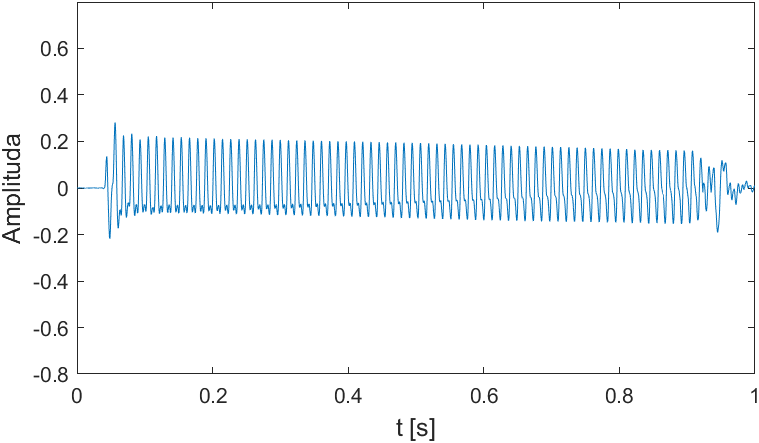
\includegraphics[width = \linewidth]{obrazky/Bass_tone_waveform.png}
        \caption{Časová oblast}
    \end{subfigure}
    \begin{subfigure}[b]{0.8\linewidth}
        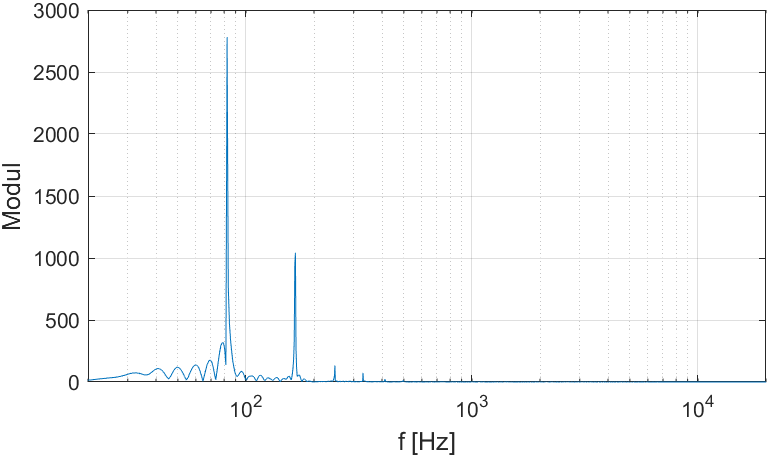
\includegraphics[width = \linewidth]{obrazky/Bass_tone_spectrum.png}
        \caption{Frekvenční oblast}
    \end{subfigure}
    \caption{Reprezentace tónu E zahraného na basovou kytaru.}
    \label{fig:Bass_tone}
\end{figure}
  
  Jako nzorný důvod proč je transformace do frekvenční oblasti přínosná je dán příklad. Na nástroj je zahrán tón, který je nahrán. 
  V časové oblasti je možné určit délku tónu a jeho průběh podle ADSR obálky popsané v bodě č. \ref*{sec:Barva}.
  Pokud je ale potřeba zjistit výšku tónu a určit notu, tak je to téměř nemožné.
  Díky transformaci do frekveční oblasti je patrná fundementální harmonická frekvence tónu.
  Tato frekvence udává výšku tónu a je tak možné stanovit notu která byla zahrána.

  Pro získání frekvenčního spektra signálu je třeba transformovat signál s časové oblasti.
  K tomu se využívá \textbf{Fourierovy transformace}. 

  Hlavní pilířem Fourierovy transformace je, že každý periodický signál je možné rozložit na součet někonečně mnoha sinusových signálů s různou amplitudou a fází.
  Toho je poté pomoí matematickýh postupů docílit.
  Analyzující signál je rozložen na jeho frekvenční složky udávané amplitudou a fází viz obrázek č.\ref*{fig:Bass_tone}.
  Jako další grafické zobrazení časové oblasti hudebního signálu se pro jeho analýzu využívá spektrogramu.
  % Spektrogram zobrazuje frekvenční složky signálu v závislosti na čase. Modul těchto složek je pak udáván barevnou škálou.
  % Spektrogram je zobrazen na obrrázku č. %TODO: popsat spektrogram zde nebo jinde? a popsat? 


  \subsection{DFT - Diskrétní Fourierova transformace}

  Pokud jsou signály zpracovávány pomocí výpočetních procesorů,
  tak může být uložen pouze omezený počet parametrů signálu.
  To znamená, že analogový signál spojitý v čase musí být převeden na signál digitální tvz. signál diskrétní, který je není spojitý v čase. 
  Diskrétní signál je potom vhodný pro číslicové zpracování.
  Důsledkem toho bylo nutné odvodit algoritmus \acs{DFT} přizpůsobený právě pro zpracování diskrétních signálů s konečným počtem hodnot.

  \begin{figure}[H]
    \centering
    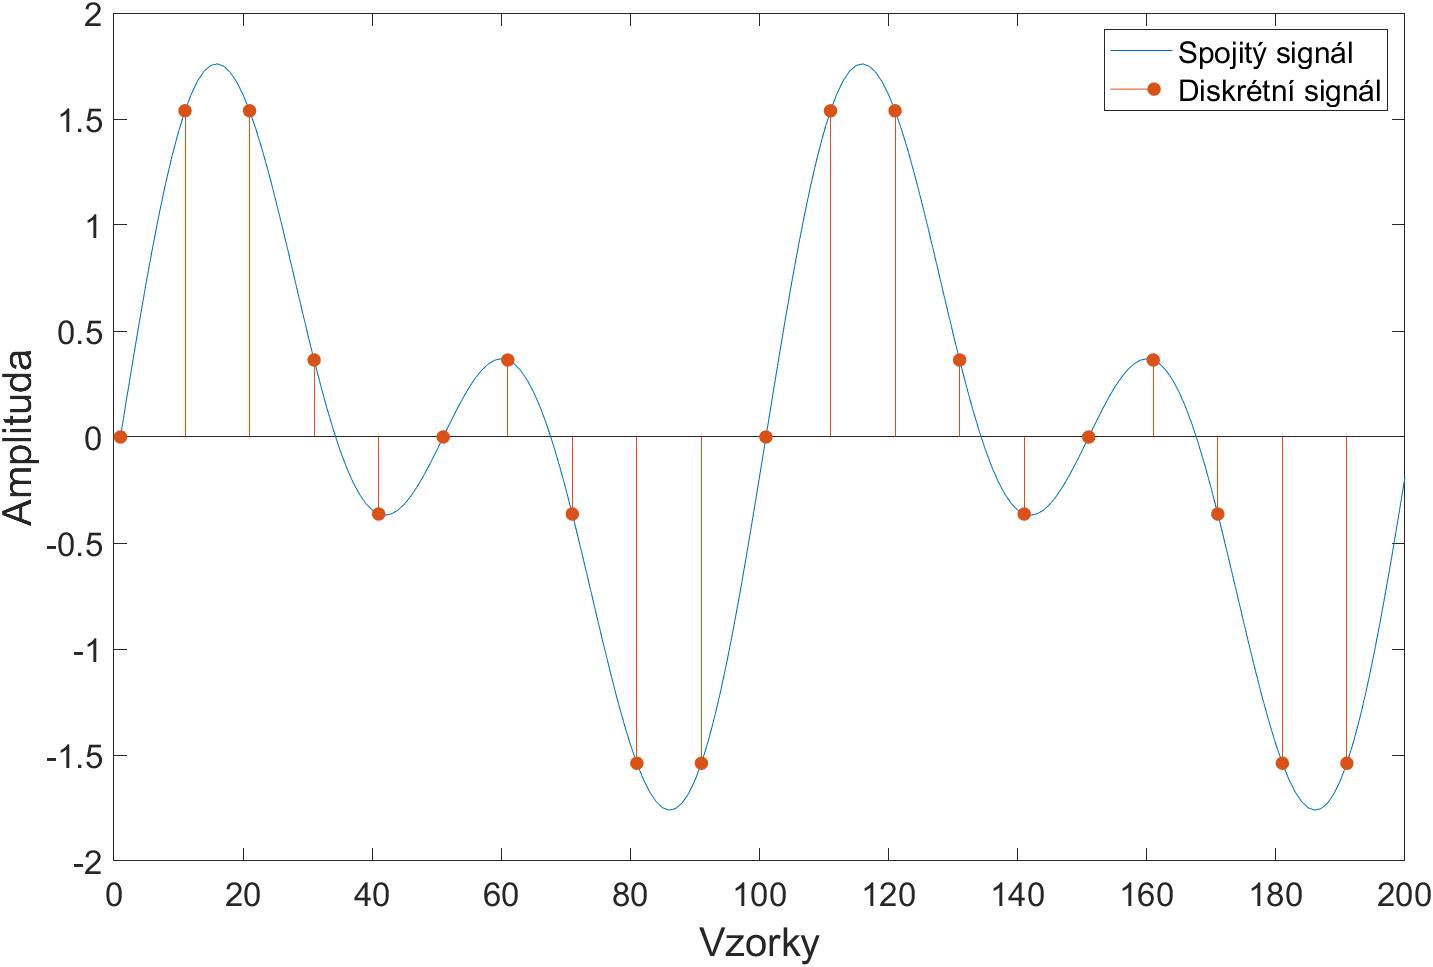
\includegraphics[width = 0.8\linewidth]{obrazky/Discrete_signal.png}
    \caption{Časově spojitý signál a diskrétní signál}
    \label{fig:Discrete_signal}
  \end{figure}

  Rovnice pro \acs{DFT} je potom zapsána v následujícím tvaru. 

  \begin{equation}
    X(k) = \hat{x}(k/N) = \sum_{n = 0}^{N - 1} x(n) exp(-2 \pi i k/N)
    \label{rov:DFT}
  \end{equation}

  Kde $ k \in [0:M - 1] = [0:N - 1] $ a $ M \in \mathbb{N}$.

  Ze strany výpočetní náročnosti je takto definovyný algoritmus neefektivní a výpočetně náročný.
  Při počítání Fourierova koeficientu $X(k)$ je zapotřebí velkého množství velké množství operací v řádu $N^2$.
  Proto pokud počet vzorků $N$ dosahuje většího množství je ve většině případů tento algoritmus příliš pomalý pro praktické využití.

  Počet potřebných operací může být výrazně redukován použitím efektivního algoritmu známého jako \acs{FFT} (\acl{FFT}).
  Na vytvoření\acs{FFT} se zasloužil Carl Friedrich Gauss a Joseph Fourier zhruba před dvěma sty let.
  Vynález tohoto algoritmu změnil své odvětví zpracování signálů a je dnes používán v miliardách telekomunikačních zařízeních.
  Ačkoliv je ve velké míře využíván v telekomunikacích, tak právě i ve zpracování a analýze zvukových signálů zabírá důležitou roli.

  Zjednodušeně \acs{FFT} využívá redundace napříč sinusovými signály různých frekvencní ke společnému výpočtu všech Fourierových koeficientů pomocí rekurze.
  Díky tomu je dosaženo snížení výpočetní náročnosti počtu operací z řádu $N^2$ na $N\log_2 N$.
  Například při použití vzorků $N = 2^10 = 1024$. \acs{FFT} vzžaduje $N\log_2N = 10240 $ operací namísto
  $N^2 = 1048576$ operací při použití \acs{DFT}. Jak je vidět snížení výpočetní náročnosti je velké a exponenciálně roste s větším počtem vzorků $N$.
  
  \subsection{STFT - Short-time Fourier transform}

  V roce 1946 Dennis Gabor představil \acs{STFT} jako potřebu zařazení frekvenčních složek do konkrétnímo času signálu.
  Fourierova transformace umožňovala převod signálu z časové oblasti do frekvenční ale nebylo zřejme v jakém časovém úseku signálu se získané fekvenční složky nachází.
  Hlavní myšlenkou \acs{STFT} je, že namísto analyzování celého signálu je signál analyzována pouze jeho malá část.
  Za tímto účelem je definována tzv. okénokvá funkce, která je nenulové pouze v malé části signálu.
  Analyzovaný signál je následně vynásoben vzniklou okénkovou funkcí a díky tomu vzniká malá nenulová části signálu dle okénkové funkce viz obr č. \ref*{fig:princip_stft}.
  Chceme li analyzovat signál v různých časech je tato funkce po signálu posouvána a následně se počítá Fourierova transformace pro každý výsledný okénkový signál.

  \begin{figure}[H]
    \centering
    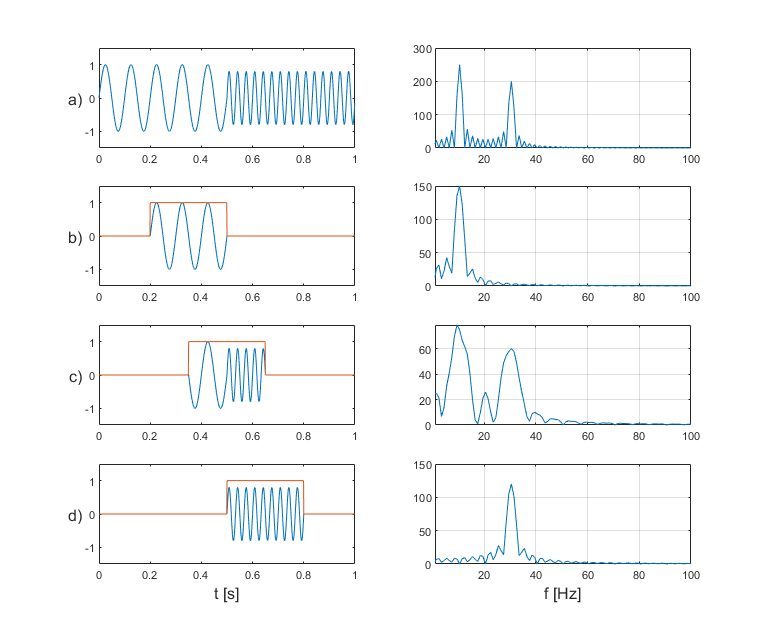
\includegraphics[width = 1\linewidth]{obrazky/STFT.png}
    \caption{Signál o délce $1 s$ s počáteční frekvencí $10 Hz$ a koncovou frekvencí $30 Hz$ \textbf{a)} Původní signál \textbf{b)} Signál s okénkem od $0,2 s$ do $0,5 s$ \textbf{c)} Signál s okénkem od $0,35 s$ do $0,65 s$ \textbf{d)} Signál s okénkem od $0,5 s$ do $0,8 s$};
    \label{fig:STFT}
  \end{figure}

  Na obrázku č. \ref*{fig:STFT} je graficky znázorněna myšlenka \acs{STFT}, která ukazuje výhodu přesného určení frekvenčních složek signálu v čase. 
  Signál je násoben obdelníkovou okénkovou funkcí ve třech místech.
  Tyto tři vzniklé signály jsou následně na sebe nezávazně transformovány do frekvenční oblasti.
  Z výsledků Fourierovy transformace lze vidět, že každá z těchto částí má jiné frekvenční spektrum.
  Pokud by bylo zapotřebí například určit přesný přechod mezi dvěma frekvencemi nacházejícími se v signálu. Lze spřesnit časové měřítko analýzy pomocí délky okénka.
  Tím ale dochází ke zmenšení přesnosti ve frekvenční oblasti.
  
  Na výsledku přesnosti analýzy poomcí \acs{STFT} závisí také tvar použité okénkové funkce.
  V obrázku č. \ref*{fig:STFT} je použito obdélníkového okénka které díky svým ostrým hranám zkresluje výsledek o nechtěné frekvenční složky.
  Existuje více tvarů okénkových funkcí pro odstranění nežádoucích složek.
  Například to jsou Kaise, Chebyshev, Hann a Haming a další.
  \cite{Time-frequency_distributions};

  %TODO: popsat parametry z knížky: dynamika intenzita a hlasitot, barva

  \subsection{Dynamika intenzita a hlasitost} \label{sec:Frekvence}

  Pojem \textbf{dynamika} je vyjadřuje jak hlasitost \uv{volume} zvuku stejně jako v notovém zápise udává hlasitost \uv{volume} přednesu.
  V notovém zápise je dynamika popsána symboly jako jsou například pianissimo \uv{\emph{pp}}, piano \uv{\emph{p}}, forte \uv{\emph{f}} a další.

  Naopak ve audiu je dynamika udána \textbf{hlasitostí \uv{loudness}} představována apmlitudou signálu nebo jeho efektivní hodnotou \acs{RMS} v čase.
  Při měření hlasitosi je pak využíváno pojmů \textbf{intenzita} zvuku a \textbf{akustický výkon}.
  Kde akustický výkon je definován jako kolik energie je vzduchem vyzářeno zvukovým vysílačem za jednotku času. Jednotkou je $[W]$
  A intenzita zvuku pak je definována jako množství energie, které projde jednotkovou plochou kolmou na směr šíření na jednotku času. Jednotkou pak je $[Wm^{-2}]$ \cite{intenzita_zvuku_definice}
  
  Z pohledu vnímání hlasitosti lidským uchem je rozsah vnímané intenzity zvuku v řádech bilionů. Práh slyšení činí $10^{-12} Wm^{-2}$ a práh bolesti je $10 Wm^{-2}$.
  Pro zmenšení tak velkého řádu je definována hladina intenzity zuvku v decibelech [$\textbf{dB}$]. Kde vztažnou hodnotou je práh slyšení $I_0 = 10^{-12} Wm^{-2}$.
  Hladina intenzity se vypočítá dle rovnice č. \ref*{rov:hladina_intenzity}

  \begin{equation}
    L_I = 10*log(\frac{I}{I_0})
    \label{rov:hladina_intenzity}
  \end{equation}
  \subsection{Barva} \label{sec:Barva}

  Jedním z důležiitých nástrojů pro jeho nalaýzuj je určení obálky signálu.
  %TODO: Popsat ADSR obálku

\section{Detekce tempa a dob}
\section{Klasifikace žánrů a nálady}

\section{Systém Spectoda}

\section{Hudební signál jako animace}

%%% Vložení souboru 'text/vysledky' s popisem vysledků práce
% (rozdělte na více souborů či kapitol, pokud je vhodné)
\chapter{Výsledky studentské práce}

% Referenční skladby http://isophonics.net/about

\section{Návrh výsledného systému}

Návrh popisuje komplexní systém skládající se z několika částí, uživatelské rozhraní algoritmů pro získání pamrametrů hudební nahrávky a algoritmu generujícího SpectodaCode na základě získaných parametrů. V této kapitole je podrobně popsán návrh jednotlivých částí systému. 

\subsection{Uživatelské rozhraní}

Uživatelské rozhraní je reprezentováno webovou stránkou a je naprogramováno pomocí značkovacího jazyka \acs{HTML} spolu s formátováním v jazyce CSS. Funkčnosto webové stránky je zajištěna funkcemi jazyce JavaScript. Javascript také vytváří propojovací můstek pro komunikaci s vnistřním systémem v jazyce Python.

Jedná se o jednoduché webové rozhraní ve kterém uživatel nahraje hudební skladbu ve formátu .wav. Rozhranní obsahuje pole pro vložení cesty k hudební skladbě umožňující výběr ze souborů v uživatelově uložišti. Níže je posuvník s 4 základními hodnotami pro výběr nálady
\uv{mood}. Jedná se hodnoty \uv{chill}, \uv{hang out}, \uv{feeling happy} a \uv{dancing}, které jsou v tomto pořadí na posuvníku. Uživatel může pomocí posouvání posuvníku vybrat pro jakou náladu chce vytvořit animaci. Pod posuvníkem pro výběr nálady se nachází tlačítko pro spuštění procesu generování SpectodaCodu.
Poslední částí webového rozhraní je textové pole ve kterém se zobrazí vygenerovaný SpectodaCode.

 \begin{figure}[H]
    \centering
    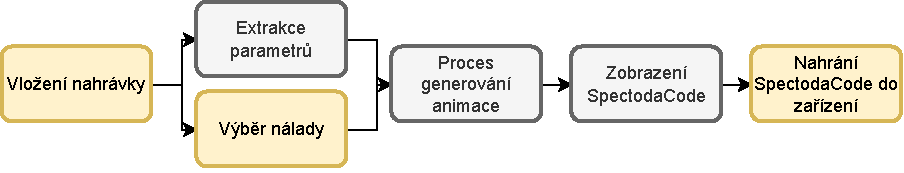
\includegraphics[width = 1\linewidth]{obrazky/User_interaction_diagram.pdf}
    \caption{Blokové schéma postupu uživatele webovou stránkou}
    \label{fig:User_interaction_diagram}
\end{figure}

Na blokovém schématu \ref{fig:User_interaction_diagram} je zobrazen proces postupu uživatele skrze webové rozhraní. 

\subsection{Parametry hudební nahrávky} \label{sec:Parametry_nahravky}

Systém popsaný v bodě \ref{sec:System_generovani_animaci} vyžaduje vstupní data o hudební nahrávce. Tyto data jsou rozdělena 7 odlišných objektů. Každý z těchto objektů představuje určitou vlastnost analyzované nahrávky. Tyto vlastnosti jsou získány pomocí technik popsaných v bodě \ref{sec:Exktrakce_vlastnosti_metody}. Jednotlivé vlastnosti a jejich datové struktury jsou shrnuty v následujících bodech.

\begin{description}
    \item[Detekce dob] představuje pole hodnot jehož délka je závislá na době trvání nahrávky. Jednotlivé hodnoty pak udávají časy hudební nahrávky, ve kterých se nacházejí doby.
    \item[Tempo skladby] je číslo typu float s jednotkou \acs{BPM} vyjadřující počet úderů za minutu. Hodnota BPM se vztahuje k počtu čtvrťových not za minutu. Vybraný algoritmus s knihovny Librosa ovšem nedetekuje jestli se jedná o noty čtvrťové. Postup zjištění tempa je popsán v bodě \ref{Librosa}.
    \item[Chromavektory] jsou získány v podobě pole jehož počet řádků udává 12 půltónů rozdělujících 1 oktávu. Délka pole je závislá na délce nahrávky a velikosti okna  při výpočtu \acs{STFT}. K matici chromavektorů je přidáno pole o stejné délce. Hondonty v poli udávají čas konce okna, ve kterém jsou počítány chroma vlastonsti. Tyto dvě proměnné jsou zadány jako parametry třídy s názvem $ChromaVector$ jehož struktura je zobrazena v blokovém schématu \ref{fig:ChromaVector_class_diagram}.

    \begin{figure}[H]
        \centering
        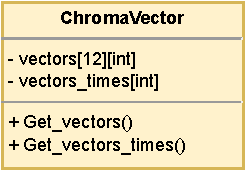
\includegraphics[width = 0.3\linewidth]{obrazky/UML_diagram_ChromaVector.pdf}
        \caption{Struktura třídy $ChromaVector$}
        \label{fig:ChromaVector_class_diagram}
    \end{figure}

    \item[Efektivní hodnota signálu] je zapsána třídou $Loudness$ obsahující dva atributy. Prvním z nich je pole $rms$ jehož délka je závislá na délce signálu a obsahuje efektivní hodnoty signálu v časech uložených v druhém atributu. Druhý atribut $times$ je pole o stéjné délce jako pole s hodnoty rms a obsahuje časy skladby ve kterých je hodnota rms počítána. 
    
    \begin{figure}[H]
        \centering
        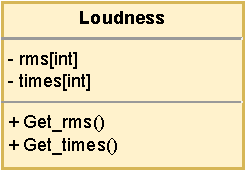
\includegraphics[width = 0.3\linewidth]{obrazky/UML_diagram_Loudness.pdf}
        \caption{Struktura třídy $Loudness$}
        \label{fig:Loudness_class_diagram}
    \end{figure}

    \item[Segmentace] je zapsána jako pole objektů tířdy $Segment$. Tato třída obshahuje 3 atributy $type$, $start\_time$ a $end\_time$. Argument $type$ obsahuje statickou hodnotu označující o jakou část skladby se jedná. Tyto hodnoty jsou vypsány v úryvku kódu \ref{code:song_segments_variables}.
    Argumenty $start\_time$ a $end\_time$ označují začátek a konec segmentu v nahrávce. 

    \begin{figure}[H]
        \centering
        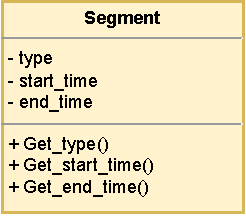
\includegraphics[width = 0.3\linewidth]{obrazky/UML_diagram_Segment.pdf}
        \caption{Struktura třídy $Segment$}
        \label{fig:Loudness_Segment_diagram}
    \end{figure}
    \begin{lstlisting} [
        caption = {Hodnoty proměnné $type$},
        captionpos=b,
        label = {code:song_segments_variables}]
        # Song segments variables
        SILENT      = 0
        REFRAIN     = 1
        STROPHE     = 2
        BRIDGE      = 3
    \end{lstlisting}

    \item[Žánr] představuju proměnou $genre$ typu short vekteré je zapsáno číslo označující žánr skladby. Statické hodnoty žánrů jsou zapsány v úryvku kódu \ref{code:song_genre_variables}.
    \begin{lstlisting} [
        caption = {Hodnoty proměnné $genre$},
        captionpos=b,
        label = {code:song_genre_variables}]
        # Song genre variables
        CLASSIC     = 0
        FOLK        = 1
        POP         = 2
        ROCK        = 3
        METAL       = 4
        ELECTRONIC  = 5
    \end{lstlisting}
    \item[Nálada] představuje proměnou $mood$ typu float s přednastavenými statickými hodnotami zobrazenými v části kódu \ref{code:song_mood_variables}. Nálada může být i v rozmezí přednastavencýh hodnot. V tomto případě je výsledná hodnot lineráně závislá na vzdálenosti od přednastavených hodnot. 
    \begin{lstlisting}[
        caption = {Hodnoty proměnné $mood$},
        captionpos=b,
        label = {code:song_mood_variables}]
        # Song mood variables
        CHILL       = 0
        HANG_OUT    = 1
        HAPPY       = 2
        DANCING     = 3
    \end{lstlisting}
    
\end{description}

\subsection{Systém pro generování animací} \label{sec:System_generovani_animaci}

Systém pro generování animací představuje nejduležitější část práce. Jeho struktura udává vizuální kvalitu animací a schopnost přizpůsobit se daným skladbám růtzných žánrů. V této kapitole je popsána základní struktura systému. 

První částí systému je vstupní rozhraní, ve kterém jsou přijímány data obsahující paramery o hudební nahrávce. Struktura přijímaných dat je popsána v budě \ref{sec:Parametry_nahravky}. Každý ze zmíněných parametrů plňí důležitou funkci v rozhodovacím procesu skládání bloků animace. Níže jsou popsány rozhodovací funkce pro jednotlivé parametry.

\begin{description}
    \item[Žánr a nálada] jsou používány pro výběr vhodného balíčku animací. Tyto balíčky jsou nazývány datasety a jejich datová struktu je popsána v bodě \ref{sec:Database_structure}. Źánr i nálada jsou zaznamenány jako předdefinovaná celočíslená hodnota. Postup výběru datasetu je následující. Každý dataset obsahuje seznam žánrů pro který je vhodný. Na základě proměnné $genre$ dochází k výběru všech datasetůch vhodných pro daný žánr. Následně na základě proměnné $mood$ ve které je uložená nálada je vabráno 5 datasetů s nejbližší hodnotou $mood\_characteristic$.
    
    \begin{figure}[H]
        \centering
        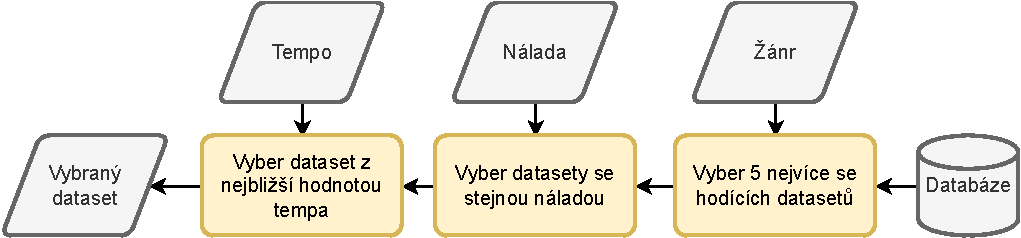
\includegraphics[width = 1\linewidth]{obrazky/Dataset_selection_diagram.pdf}
        \caption{Blokový diagram výběru datasetu.}
        \label{fig:Dataset_selection_diagram}
    \end{figure}

    \item[Tempo skladby] je posledním parametrem při výběru vhodného datasetu. 
    Hodnota proměné $speed\_suitability$ každého z 5 vybraných datasetů je porovnána s tempem skladby. Finální dataset je vybrán ten jehož hodnota $speed\_suitability$ je nejbližší hodnotě tempa skladby. Blokový diagram procesu je znázoprněn na obrázku \ref{fig:Dataset_selection_diagram}. Tempo skladby je také použito pro výpočet délky jednotlivých animací na které je přímo úměrná rychlost animace. Tento postup je více popsán níže. %TODO: připadt referenci na část kde je popsán výpočet délky animace.
    \item[Segmentace] slouží pro detekci opakujících se částí nahrávky. Například nahrávka obsahuje více než jednu sloku či refrémů.Je kladen důraz aby v opakujících sesegmentec nahrávky byla animace stejného typu. Z toho plyne, že v každém refrému bude podobná animace.
    \item[Detekce dob] je základní parametrem na základě kterého se nastaví začátky a konce animací tak, aby odpovídaly rytmu nahrávky.
    \item[Chroma vektory] udávají tónovou strukturu skladby v průběhu času. Tento parametr je využit pro nastavení barevné škály animací. Chromavektory se analyzují a jsou vybrány 4 hlavní tóny nejčastěji se vyskytující v nahrávce. Keždému tónu je přiřazen barevný odstín. Poté je animaci v dané části skladby přiřazena barva dle tónu určeném chromavektorem daného času nahrávky.
    %TODO:Blokové schéma?
    \item[Efektivní hodnota signálu] pomáha procesu segmentace. Refrém a sloka se mohou lyšit hlasitostí která je zpjata se efektní hodnotou. Zároveň je použita pro výběr vhodného typu animace. Na základě velikosti efektivní hodnoty signálu v čase je vybrán typ animace. Vyžší hodnoty představují rychlejší a údernější animace. Nižší hodnoty naopak pomalejší a klidnější animace. Tento procej je zajištěn porovnáváním proměné $anim_characteristic$ obsažené v každém bloku animace s efektivní hodnotou mapovanou na určený rozsah.
    %TODO: Vymyslet a pospat proces mapování efektivní hodnoty. 
    %TODO: Popsat tak aby to odpovídalo struktuře anim_characteristic dle blokového diagramu.
\end{description}

\
Druhá část systému tvoří samotnou logiku skládání blkoků animací. Tato rozhodovací struktura je zobrazena na blokovém diagramu.

\begin{figure}[H]
    \centering
    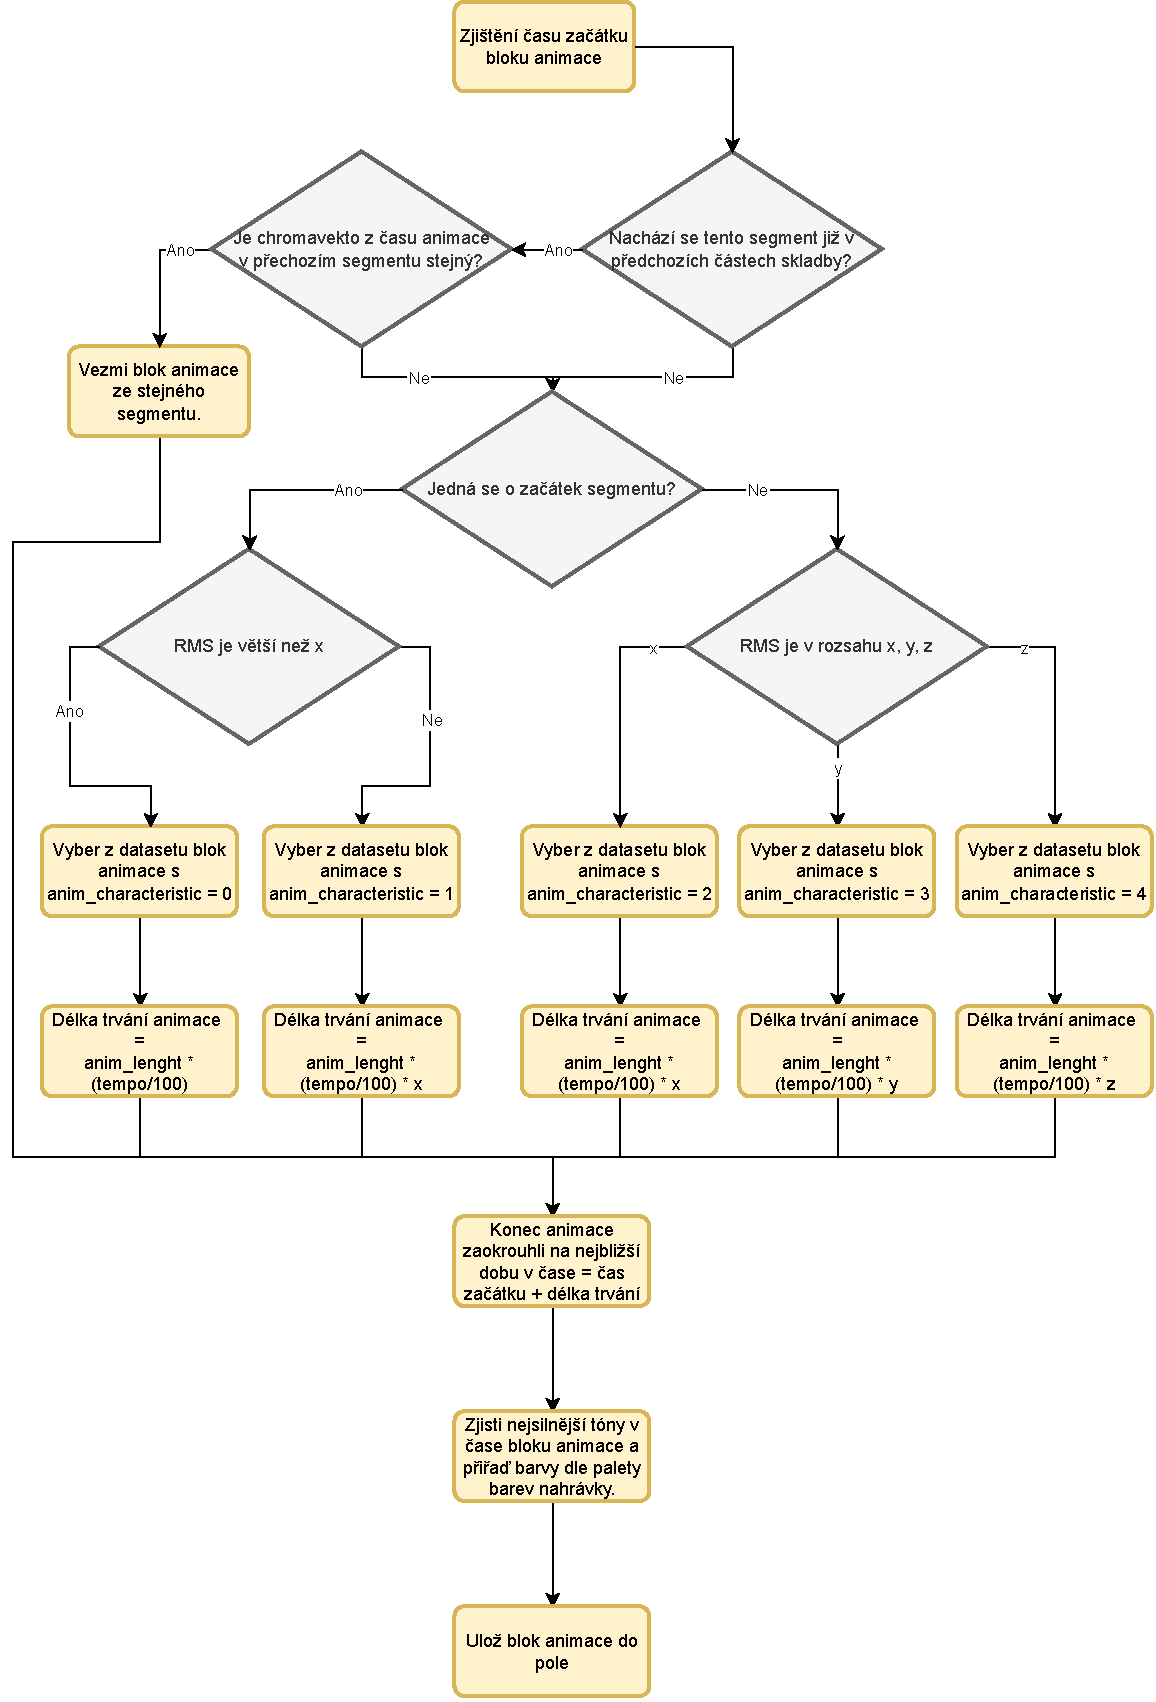
\includegraphics[width = 1\linewidth]{obrazky/Logical_structure_diagram.pdf}
    \caption{Blokový diagram rozhodovací struktury.}
    \label{fig:Logical_structure_diagram}
\end{figure}

% Na začátku je zjištěno jestli se jedná o první blok animace. Pokud ano je nastaven čas začátku animace jako čas první doby v nahrávce. Jestli se nejedná o první blok animace, tak je nastaven čas začátku jako konec předchozího bloku animace. Tento proces v blokovém schématu \ref{} představuje proces s názvem \uv{Nastavení času začátku animace}. Druhým krokem je rozhodovací struktura jestli se vybraný čas začátku nachází v segmentu nahrávky který se opakuje. Pokud ano je nalezen blok animace ve stejném času předchozího segmentu a je zkontrolováno  


\subsection{Databáze bloků animací} \label{sec:Database_structure}
Jak je popsáno v bodě \ref{sec:Spectoda}...

%TODO: Popsat Dataset atd...


\section{Výběr vhodných metod pro extrakci vlastností hudební nahrávky} \label{sec:Exktrakce_vlastnosti_metody}

Vědeská komunita nabízí několik volně šířících knihoven obsahující techniky z oborů MIR. V této části práce jsou prozkoumány 3 knihovny zmíněné v bodě \ref{sec:Dostupna_reseni}. Jsou použity jejich funkce získání potřebných parametrů hudební nahrávky potřebných pro navazující diplomovou práci. Tyto funkce jsou mezi sebou porovnány z hlediska přesnosti výsledků, rychlosti výpočtů, jednoduchosti použití a možnosti využití pro komerční účely. 

\subsection{Detekce dob a tempa}

\subsection{Analýza chromavektorů}

\subsection{Efektivní hodnota signálu}


Vstupními parametry systému jsou získané parametry jež jsou popsány v bodě \ref{sec:Parametry_nahravky} 

% Možná lepší první popsat strukturu systému jak by se měly animace generovat a co k tomu budou potřeba za parametry. Následně teprve vytvořit sekci kde je popsán vzniklý kód pro analýzu jednotlivých parametrů. Také důležité jestli ukázaky kódu atd.. nebudou zahrnuty spíše v sekci Věběr vhodných metod pro extrakci vlastností hudební nahrávky. 

%%% Vložení souboru 'text/zaver' se závěrem
\chapter*{Závěr}
\phantomsection
\addcontentsline{toc}{chapter}{Závěr}

%Shrnutí studentské práce co jsem dělal a musí zaznít co budu dělat v diplomové práci a jak toho dosáhnu.


V rámci semestrální práce byla prozkoumána vědní oblast \acs{MIR}, metody vzniklé v rámci výzkumů v této oblasti a možnost jejich využití pro navazující diplomovou práci. Komunita soustředící se kolem oblasti \acs{MIR} vytvořila pro vědecké účely volně dostupné knihovny. Tyto knihovny jsou lehce implementovatelné v programovacím jazyce python a obsahují pokročilé mteody pro analýzu a práci s hudebními nahrávkami v časové i frekvenční oblasti.

V první části \ref{sec:Teorie} je popsána teorie základních principů práce s hudební nahrávkou v digitální formě. Od metod využívajícíh základní principy zpracování signálů po moderní řešení s využitím strojového učení. Dále jsou v této části v bodech \ref{sec:Librosa} až \ref{sec:Mir_eval} popsány víše zmíněné dostupné knihovny jejich metody pro extrakci parametrů, potřebných pro navazující diplomovou práci, a principy jak jsou tyto metody realizovány.

Výsledkem semestrální práce je návrh systému pro generování SpectodaCodu na základě parametrů nahrávky. SpectodaCod je následně nahrán do Spectoda zařízení, které kód převádějí na světelné animace. Návrh systému je rozdělen na několik částí. Uživatelské rozhraní popsané v bode \ref{sec:User_interface}, parametry potřebné pro realizaci funkčního procesu generování animací a popis jejich datové struktury je v bodě \ref{sec:Parametry_nahravky}. Popis jak by celý proces generování měl v principu fungovat a jeho struktura je popsána v bodě \ref{sec:System_generovani_animaci}.

Posledním bodem práce byla samotná extrakce vybraných parametrů z hudební nahrávky. Jsou prozkoumány dostupné metody a vytvořeny Jupyter notebooky, jež jsou k nalezení v příloze práce, obsahujících porovnání těchto metod na základě přesnosti a rychlosti výpočtů. Hodnocena je také vhodnost pro výsledný systému. Tato část práce je popsána v bodě \ref{sec:Exktrakce_vlastnosti_metody}.

V rámci navazující diplomové práce dojde k realizaci výsledného systému a jeho uvedení do funkčního stavu. Bude naprogramováno uživatelské rozhraní popsané v bodě \ref{sec:User_interface} a realizována rozhodovací struktura zobrazena v budě \ref{sec:System_generovani_animaci}. Tato struktura bude následně testována a upravena, aby bylo dosaženo funkčního generování vizuálně zajímavých animací. Na základě existence rozhodovací struktury dojde k přezkoumání vhodnosti získaných parametrů a jejich úprava pro lepší výsledky při generování animací. 

%Není zde popsána segmentace, která zatím není realizována stejně jako přidělování žánrů. 

% Bude doplněna teorie ke knihovnán Madmom, Aubio a Mir_eval


%%% Vložení souboru 'text/literatura' se seznamem zdrojů

%%2) Seznam citací pomocí BibTeXu
%% Při použití je nutné v TeXnicCenter ve výstupním profilu aktivovat spouštění BibTeXu po překladu.
%% Definice stylu seznamu
\bibliographystyle{czechiso/czechiso}
%% Pro českou sazbu lze použít styl czechiso.bst ze stránek
%% http://www.fit.vutbr.cz/~martinek/latex/czechiso.tar.gz
%% Vložení souboru se seznamem citací
\bibliography{text/literatura}
%
%% Následující příkaz je pouze pro ukázku sazby literatury při použití BibTeXu.
%% Způsobí citaci všech zdrojů v souboru literatura.bib, i když nejsou citovány v textu.

%%% Vložení souboru 'text/zkratky' se seznam použitých symbolů, veličin a zkratek
\cleardoublepage
\chapter*{\listofabbrevname}
\phantomsection
\addcontentsline{toc}{chapter}{\listofabbrevname}

\begin{acronym}[KolikMista]
	\acro{MIR}
		{Music information retrieval - Obor zabývsjící se vyhledávání informací v hudebních dílech}
	
	\acro{MIDI}
		{Musical Instrument Digital Interface - Digitální rozhraní hudebních nástrojů}

	\acro{ISMIR}
		{International Society of Music Information Retrieval - Mezinárodní združení pro \acs*{MIR}}	

	\acro{MIREX}
		{The Music Information Retrieval Evaluation eXchange}
		
	\acro{FFT}
		{Fast Fourier transform - Rychlá Fourierova transformace}

	\acro{DFT}
		{Discrete Fourier transform - diskrétní Fourierova transformace}

	\acro{STFT}
		{Short-time Fourier transform - krátkodobá Frourierova transformace}
	
	\acro{RMS}
		{Root mean square - efektivní hodnota}
\end{acronym}


%%% Začátek příloh
\appendix

%%% Vysázení seznamu příloh
% (vynechejte, pokud máte dvě nebo méně příloh)
% \listofappendices

%%% Vložení souboru 'text/prilohy' s přílohami
% Obvykle je přítomen alespoň popis co najdeme na přiloženém médiu
%\chapter{Ukázky zdrojových kódů}

\begin{minipage}{\linewidth}
	\begin{lstlisting}[
		breaklines = true,
		frame=single,
		numbers=left,
		caption={Zdrojový kód funkce \texttt{Find\_segment} v jazyce Python},
		label={code:Find_segment}]
		def Find_segment(y : list, beat_time):
		"""
		Function that finds segment from provided list in which is located the beat_time.

		Parameters
		----------
		y : list
			List of times where the segments boundaries are located
		beat_time : float
			Time of the beat which is wanted to locate.

		Returns
		----------
		start_segment : float
			Time where the located segment starts.
		end_segment : float
			Time where the located segment ends.
		"""

		y = np.asarray(y)
		idx = np.abs((y - beat_time)).argmin()

		if y[idx] > beat_time:
			idx -= 1

		start_segment = y[idx]
		try:
			end_segment = y[idx+1]
		except IndexError:
			end_segment = None

		return start_segment, end_segment

	\end{lstlisting}
\end{minipage}

\begin{minipage}{\linewidth}
	\begin{lstlisting}[
		breaklines = true,
		frame=single,
		numbers=left,
		caption={Zdrojový kód funkce \texttt{Find\_nearest\_beat} v jazyce Python},
		label={code:Find_nearest_beat}]
		def Find_nearest_beat(y : list, time):
		"""
		This function finds the nearest beat in given list.
	
		Parameters
		----------
		y : list
			List of times where the beats are located.
		time : float
			Time around that is searching for the nearest beat.
	
		Returns 
		----------
		idx : int
			Index of finded beat in the list.
		"""
		y = np.asarray(y)
		idx = np.abs((y - time)).argmin() 
		return idx

	\end{lstlisting}
\end{minipage}

\begin{minipage}{\linewidth}
	\begin{lstlisting}[
		breaklines = true,
		frame=single,
		numbers=left,
		caption={Zdrojový kód funkce \texttt{Calc\_strength} v jazyce Python},
		label={code:Calc_strength}]
		def __Calc_strength(self, onset_env):
		"""
		Calculate strength of beats.

		The function calculate beats strength based on onset envelope in time of the beat. Function also check range around the beat if there is some bigger value in onset envelope.

		Parameters
		----------
		onset_env : ndarray
			Onset envelope
		"""
		self.__strength = np.ones(len(self.__beats)) # Declaration of ones ndarray.
		i = 0

		for beat in self.__beats:
			try:
				index = np.where(self.__times == beat)[0] # Getting a timestamp of the beat.
				self.__strength[i] = self.__Max_of_range(int(index), onset_env) # Gets a biggest onset value in range around the timestamp of beat.
			except ValueError:
				self.__strength[i] = 0
			i += 1

		self.__strength = librosa.util.normalize(self.__strength) # The beat strength normalization between values 0-1.
	
	\end{lstlisting}
\end{minipage}

\begin{minipage}{\linewidth}
	\begin{lstlisting}[
		breaklines = true,
		frame=single,
		numbers=left,
		caption={Zdrojový kód funkce \texttt{Dataset\_selection} v jazyce Python},
		label={code:Dataset_selection}]
		def Dataset_selection(dataset_database : list[Dataset], genre_classification : GenreClassification, beat_tracking : BeatTracking, mood : int):

		# Get parameters 
		genre_predictions = genre_classification.genres_predictions
		tempo = beat_tracking.tempo
		genres_difs = []
	
		# Browsing thru all datasets
		for i, dataset in enumerate(dataset_database):
			genre_dif = 0
			d_genres_prediction = dataset.genre
			for key in d_genres_prediction:
				genre_dif += d_genres_prediction[key] - genre_predictions[key]
			genres_difs.append(np.abs(genre_dif))
		genre_pass_datasets = []
	
		# Get five datasets with smallest genre difference
		for i in range(5):
			index_of_min = int(np.argmin(genres_difs))
			genre_pass_datasets.append( dataset_database[index_of_min])
			genres_difs[index_of_min] = 255
		this_tempo_dif = 100
		selected_dataset = Dataset
		
		# Get dataset with same mood an smallest tempo diference
		for dataset in genre_pass_datasets:
			if dataset.mood == mood:
				new_tempo_dif = abs(dataset.tempo - tempo)
				if this_tempo_dif > new_tempo_dif:
					this_tempo_dif = new_tempo_dif
					selected_dataset = dataset
		return selected_dataset
	\end{lstlisting}
\end{minipage}

\chapter{Obsah elektronické přílohy} \label{sec:Obsah_prilohy}
Aplikace je psaná v programovacím jazyce Python ve verzi 3.11.6. Verze použitých knihoven jsou přiloženy v textovém dokumentu s názvem \textit{package\_versions.txt}. V průběhu obhajoby práce je aplikace dostupná na webové stránce \href{http://vikinn.pythonanywhere.com/}{zde}.

\bigskip
{\small
%
\dirtree{%.
.1 /\DTcomment{kořenový adresář přiloženého archivu}.
.2 Generator\_core\_structure\DTcomment{ zdrojové kódy aplikace}.
.3 static.
.4 styles.css.
.3 templates.
.4 main\_page.html.
.3 AnimationBlock.py.
.3 BeatTracking.py.
.3 Constants.py.
.3 Dataset.py.
.3 dataset\_database.json.
.3 GenreClassification.py.
.3 ChromaFeatures.py.
.3 Main.py.
.3 Segmentation.py.
.2 Matlab\_graphs\DTcomment{zdrojové kódy grafů}.
.3 ADSR.m.
.3 Discrete\_signal.m.
.3 Energy\_function.m.
.3 FFT.m.
.3 STFT.m.
.3 Spektrogram\_tok.
.4 Mel\_spektralni\_tok.m.
.4 Spektrogram.m.
.4 Spektralni\_tok.m.
.3 Waveform.m.
.2 Method\_comparisons\DTcomment{jupyter notebooky pro porovnání extrakce parametrů}.
.3 Beat\_tracking\_comparison.ipynb.
.3 Color\_palete.ipynb.
.3 Data\_preparation.ipynb.
.3 Dataset\_creating.ipynb.
.3 GenreClasification\_02.ipynb.
.3 Chroma\_vectors\_comparison.ipynb.
.3 Segmentation.ipynb.
.3 Signal\_rms.ipynb.
.2 package\_versions.txt\DTcomment{verze použitých balíčků pro Python}.
}
}

\end{document}